%==========================================================================
%Template File for Monthly Lectual Meeting
%2006/05/22 (kkobayashi@mikilab.doshisha.ac.jp)
%==========================================================================
\documentclass[a4j,9pt,twocolumn]{jsarticle}
\usepackage{mlm2.0}
\usepackage{epsf}
\pagestyle{plain}
\usepackage{url}
\usepackage{subfigure}
\setcounter{page}{1}
\usepackage{geometry}
\geometry{left=25mm,right=25mm,top=20mm,bottom=30mm}
%\usepackage[dvips]{graphicx}

\begin{document}
\twocolumn[
%---------------------------------------------------------------------------        % ヘッダ    書式:\beginheader{回}{年}{月}
%---------------------------------------------------------------------------
\beginheader{171}{2016}{04}
%---------------------------------------------------------------------------
% 発表題目    書式:\title{日本語}{英語} 「\\」で改行できます
%---------------------------------------------------------------------------
\title%
{git}%
%{更なる大容量化を目指して 進化しつづける次世代光メディア}

%---------------------------------------------------------------------------
% 著者名      書式:\author{日本語著者名}{英語著者名}
%---------------------------------------------------------------------------
\author{山下 俊樹,外村 篤紀\\Toshiki YAMASHITA,Atsuki TONOMURA}

%---------------------------------------------------------------------------
\endheader
%\begin{abstract}
%---------------------------------------------------------------------------
%Recently, a DVD attracts attention along with the image and the digitization of the sound. The standards of these DVD are complicated. So, in this paper, the standards of the DVD are summarized and the DVD of the next generation is refered. 
%---------------------------------------------------------------------------
%\end{abstract}
]

%---------------------------------------------------------------------------
% 本文
%---------------------------------------------------------------------------

\section{はじめに}
近年,ソフトウェアの大規模化にともない,プログラムの更新頻度は増加傾向にある.そこで,コンピュータ上で作成または編集したファイルの変更履歴を管理するバージョン管理システムはより重要となっている.バージョン管理システムには,管理下のファイルを任意の記録時点の状態に復元することができることや,1つのファイルを複数人で編集する場合,競合が発生しないように管理が行えることなどの利点があるため,注目を集めている\cite{pop}.本報告では,分散型バージョン管理システムの1つであるgitの概要,バージョン管理手法,および利点について述べる.

\section{gitの構成}
gitの構成を以下の\fgref{git}に示す.

\begin{figure}[h]
\centering
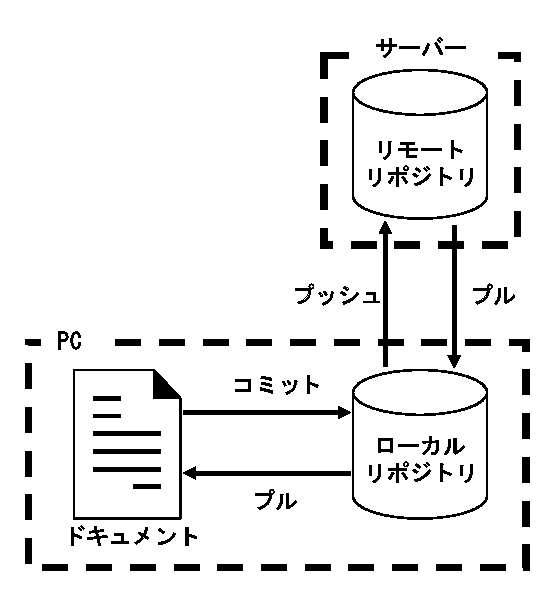
\includegraphics[width=80mm]{img/git.eps}
\caption{gitの構成}
\label{git}
\end{figure}

gitで管理されるファイルやディレクトリの変更内容は,リポジトリと呼ばれるデータベースに蓄積される.分散型バージョン管理システムにおけるリポジトリは2種類に大別できる.1つは,サーバ上に配置され複数ユーザで利用するリモートリポジトリである.もう1つは,個人のPC内に配置され,その個人が利用するローカルリポジトリである.ファイルやディレクトリの変更をローカルリポジトリに記録する操作をコミットと呼ぶ.コミットを実行すると,最新の状態が記録される.過去のコミット時点の状態への復元操作,およびブランチを切り替える操作をチェックアウトと呼ぶ.コミットやプッシュを行うことで作業成果を記録する.また,プルを行うことでリモートリポジトリから他者の作業成果をダウンロードして統合する.

\section{ブランチ}
\subsection{概要}
gitの特徴の1つであるブランチは,蓄積されたコミットの時系列を指す.すなわち,複数回のコミットを作成順に並べた連なりをブランチと呼ぶ.また,ブランチを分岐する操作もブランチと呼ぶ.分岐したブランチ同士は互いに独立しており,異なる内容の更新を同時に行える.ブランチ同士の結合はマージと呼ぶ.

\subsection{プログラム開発におけるブランチの有用性}
ブランチを利用した一例を以下の\fgref{branch_ex}に示す.

\begin{figure}[h]
\centering
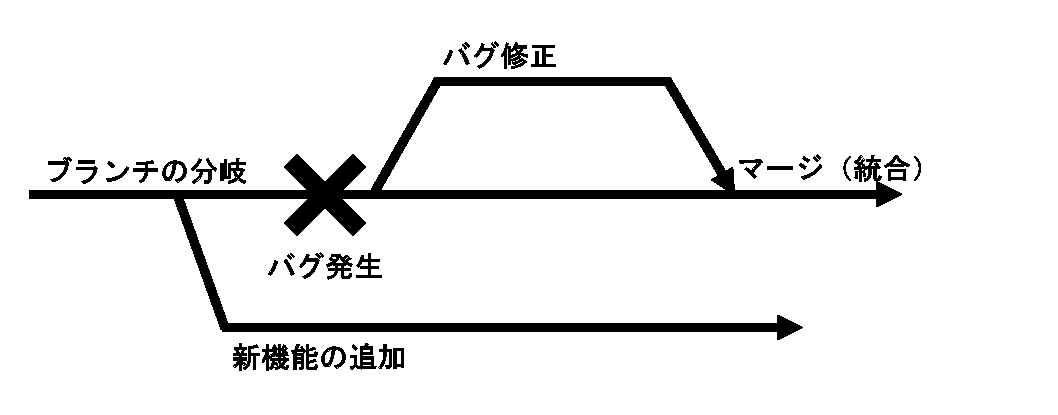
\includegraphics[width=80mm]{img/branch.eps}
\caption{ブランチの一例}
\label{branch_ex}
\end{figure}

ブランチを用いることで,様々な開発やバグ修正などを同時並行で行うことができる.\fgref{branch_ex}において既に運用されているソフトウェアの管理を行っているブランチをmasterブランチとし,そのソフトウェアのバグを修正するために用意したブランチをbugfixブランチとする.この場合,二つのブランチは独立しているため,masterブランチに影響を与えることなくbugfixブランチでバグ修正を行うことができる.すなわち,ブランチを用いない場合は,バグ修正が完了するまでソフトウェアの運用を停止しなければならない.それに対し,ブランチを用いることでソフトウェアの運用を止めることなく,平行してバグ修正を行うことができる.バグ修正が完了した後にマージを行えば,マージの時点でバグが修正される.バグ修正の間,ソフトウェアの運用は継続される.さらにブランチの本数を増やせば,リリースしたソフトウェアを運用しながら新機能の追加を行い,さらにバグ修正も同時に行うといった運用が可能である.

\section{バージョン管理手法}
\subsection{gitオブジェクト}
.gitディレクトリの構成を以下の\fgref{object1}に示す.

\begin{figure}[h]
\centering
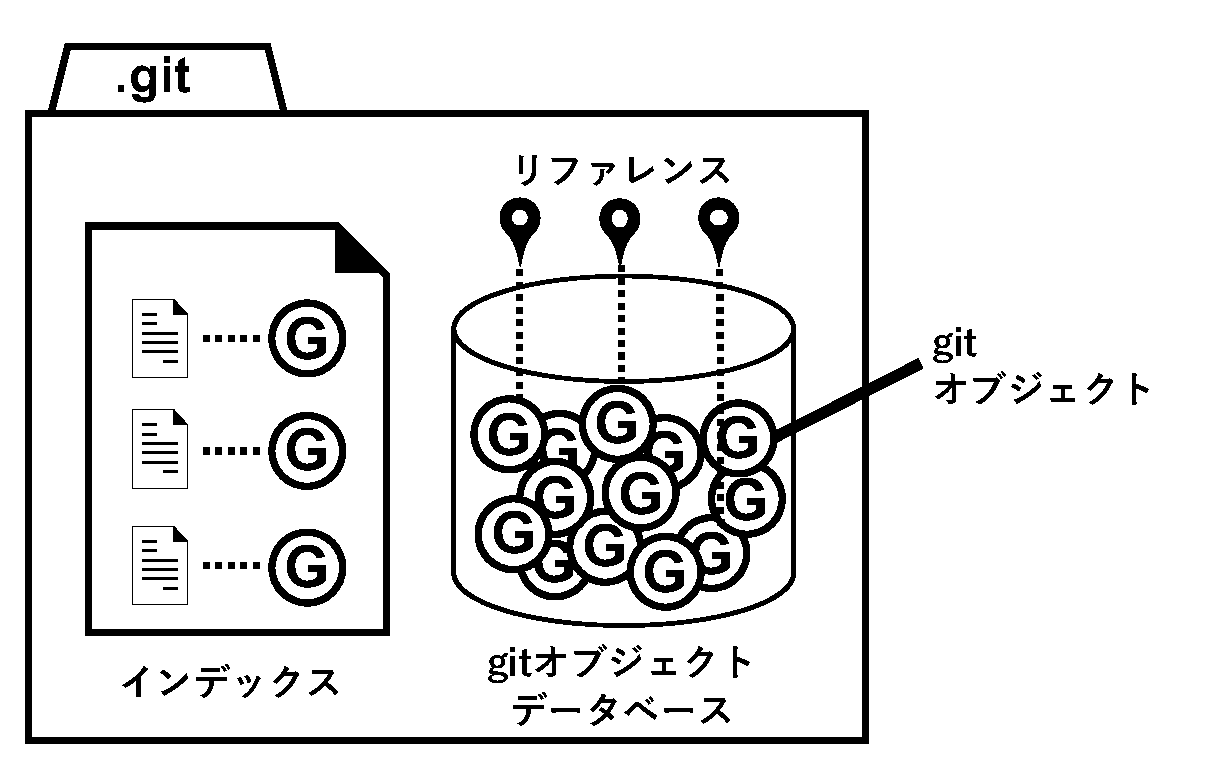
\includegraphics[width=70mm]{img/git_obj.eps}
\caption{.gitディレクトリの構成}
\label{object1}
\end{figure}

gitがどのようにバージョン管理を行っているかについて述べる\cite{mecha}.gitで管理されているディレクトリの最上層には,.gitディレクトリが生成されている..gitディレクトリがローカルリポジトリの本体である.

.gitディレクトリ内には,gitオブジェクト,リファレンス,およびインデックスが格納されている.gitオブジェクトの集合をgitオブジェクトデータベースと呼ぶ.リファレンスは各gitオブジェクトに1つずつ割り当てられる目印である.インデックスは,gitオブジェクトのデータベース内の格納位置を示している.gitオブジェクトの内容を以下の\fgref{object2}に示す.

\begin{figure}[h]
\centering
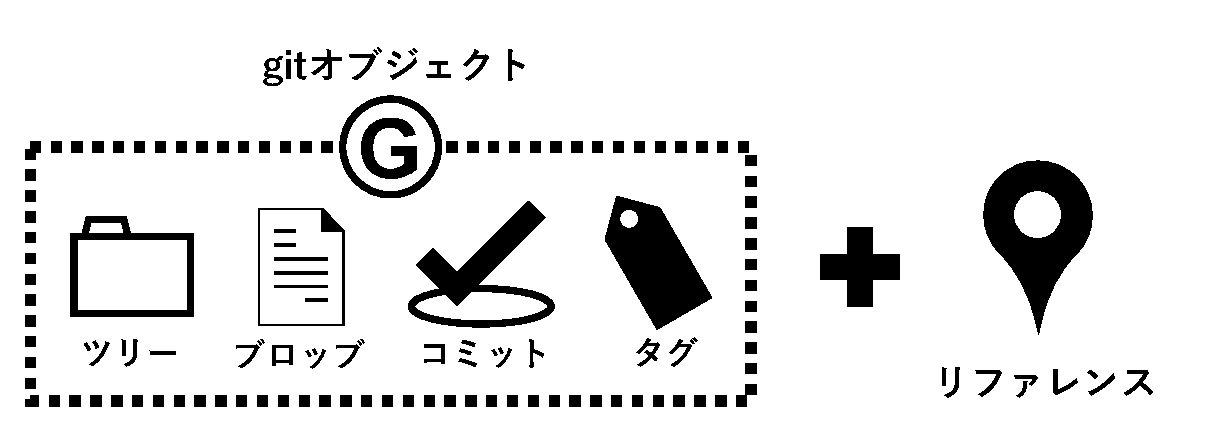
\includegraphics[width=75mm]{img/git_obj2.eps}
\caption{gitオブジェクト}
\label{object2}
\end{figure}

gitオブジェクトは4種類あり,ツリーオブジェクト,ブロッブオブジェクト,コミットオブジェクト,およびタグオブジェクトである.ツリーオブジェクトはディレクトリに相当し,ブロッブオブジェクトはファイルに相当する.gitで管理するディレクトリとファイルを,ツリーオブジェクトとブロッブオブジェクトに変換し管理する.

\subsection{ツリー}
ここで,ツリーの関係を以下の\fgref{tree}に示す.

\begin{figure}[h]
\centering
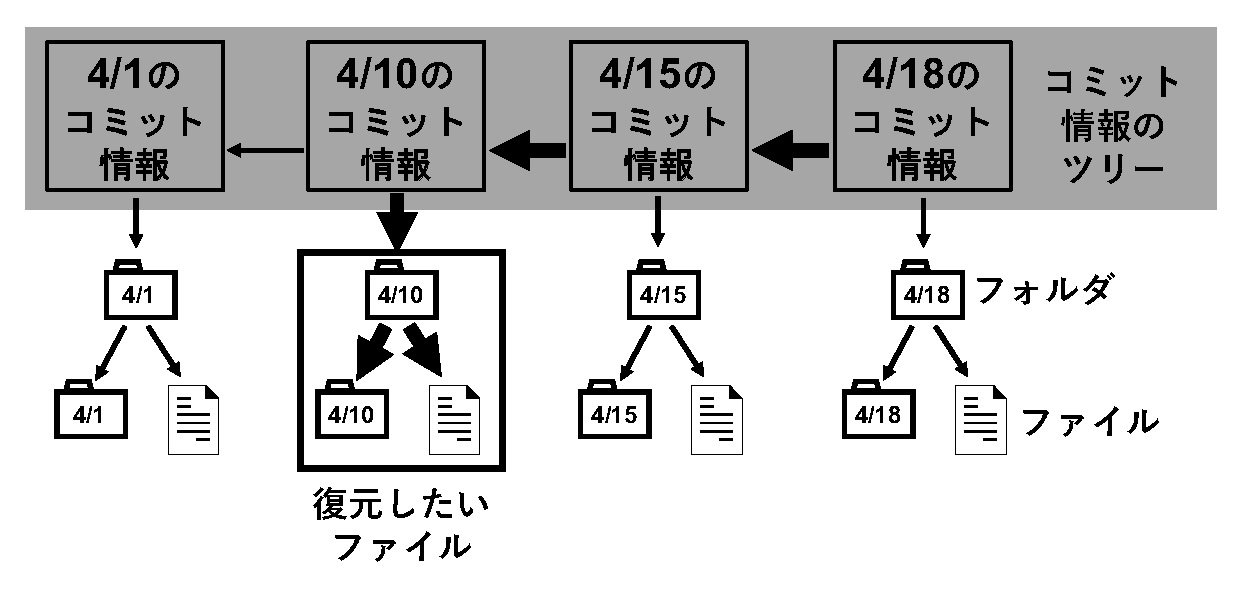
\includegraphics[width=90mm]{img/tree.eps}
\caption{ツリーの関係}
\label{tree}
\end{figure}

リファレンスは特定のコミットオブジェクトに対応し,コミットオブジェクトはツリーオブジェクト,およびブロッブオブジェクトに対応する.すなわち,リファレンスを目次として,特定のコミットの対象ファイルやディレクトリに芋づる式にアクセスできる.他にも,現在どのブランチを管理しているのかを示すリファレンスが存在し,HEADリファレンスと呼ばれる.HEADリファレンスは,リファレンスに付けられる.さらに,コミットオブジェクトには,1つ前のコミットオブジェクトへのポインタが含まれるため,コミットオブジェクトをたどることでブランチを表現できる.

コミットの時系列順の管理は,コミットツリーで行う.コミットツリーとは,コミットオブジェクト間のポインタで繋がれたツリー構造である.1つのコミットで管理される複数のファイルやディレクトリは,ファイルツリーと呼ばれるツリー構造で表される.

コミットごとにディレクトリやファイルがデータベースに蓄積する.コミットにはリファレンスを付けて管理する.さらに,コミットツリーをたどることで,過去のいかなるコミットにもアクセスすることができる.したがって,任意のコミット時点の状態に戻す場合は,リファレンスからコミットツリーをたどり,対応するファイルを取り出せばよい.

ブランチのような複雑な管理を行う場合でも,リファレンスとコミットツリーを用いて管理することにより,処理を軽減できる.その結果,git全体の動作を高速化している.差分抽出(変更点の表示)を行う場合も,対象の2つのファイルを取り出して比較を行うことで,他サービスより高速に動作する.

\section{利点と欠点}
gitは,ローカルリポジトリによって,ネットワークに接続されていない環境でもコミットを行うことができる.あるいは,バグ修正のために個人のローカルリポジトリに適量のコミットを行い,修正を完了したとする.その後,修正が完了したソフトウェアをリモートリポジトリにプッシュし,他者に公開する方法が可能である.この利点は他の分散型バージョン管理システムにも当てはまる.

さらに,ブランチ機能が他のバージョン管理システムに比べて優れている.他のシステムでは,マージの際にどのファイルをどのようにマージするか明示的に入力する必要があるが,gitは自動的に行う.また,マージにかかる時間も他のシステムに比べて高速である.

欠点は,gitで扱えるファイルの種類がテキストベースのファイルに限られる点である.このため,書類作成のデファクト・スタンダードである,Microsoft Officeで作成したファイルを改変なしでは管理できない.

\section{今後の展望}
今日,ソフトウェアのリリース速度は増加の一途を辿っている.それにともない,開発の効率化,高速化が重要視されている.そのため,gitのようなバージョン管理ソフトウェアは更に普及すると考えられる.また,GitHubのようなgitを用いたサービスは,現在概ね無料で公開されているが,あるソフトウェアの開発において,デバッグや開発の一部を他者に依頼し,一番良いソースコードを含むフォークに報酬を払うなどのビジネスも近い将来に生まれると考える.

\small
\begin{thebibliography}{99}
\bibitem{pop}
岡本隆史:Gitに潜む光と闇,入手先,(http://gihyo.jp/dev/column/01/prog/2012/git)

\bibitem{mecha}
koseki2:Git の仕組み (1),入手先(http://koseki.\\hatenablog.com/entry/2014/04/22/inside-git-1)
\end{thebibliography}
\end{document}